\chapput{intro}{Introduction}

Mainstream compilers, such as GCC\ \cite{Stallman16}, ICC\
\cite{Intel15}, and LLVM \cite{LattnerAd04} provide linguistic extensions for frameworks such as Cilk Plus\cite{IntelCilkPlus10} and OpenMP \cite{AyguadeCoDu09, OpenMP13} that allow programmers to write fork-join parallel programs. Typically in such frameworks, one can specify parallelism at a high level by denoting tasks or loops iterations that may be executed concurrently.

Although these mainstream compilers support fork-join parallelism,
they struggle to optimize programs when they encounter such linguistic constructs. 
Paradoxically this can even mean that programs you'd expect to show large parallel speedups,
are slower than the equivalant serial code. Consider, for example, the parallel \CilkFor loop on
\lirefrange{cilk_for} in \subfigref{normalize}{a}, which indicates
that iterations of the loop are free to execute in parallel.  In a
serial version of this loop, where the \CilkFor keyword is replaced by
an ordinary \code{for} keyword, each of the compilers GCC 5.3.0, ICC
16.0.3, and Cilk Plus/LLVM 3.9.0 observes that the call to \code{norm}
on \liref{normalize_element} produces the same value in every
iteration of the loop, and they optimize the loop by computing this
value only once before the loop executes.  This optimization
dramatically reduces the total time to execute \code{normalize} from
$\Theta(n^2)$ to~$\Theta(n)$.  Although
this same optimization can, in principle, be performed on the actual
parallel loop in the figure, no mainstream compiler performs this
code-motion optimization.  The same is true when the parallel loop is
written using OpenMP, as shown in \subfigref{normalize}{b}.

This failure to optimize stems from how these compilers for serial
languages implement parallel linguistic constructs.  The compiler for
a serial language, such as C \cite{KernighanRi88} or C++
\cite{Stroustrup13}, can be viewed as consisting of three phases: a
front end, a middle end, and a back end.  The front end parses and
type-checks the input program and translates it to an
\defn{intermediate representation (IR)}, which represents the control
flow of the program as a more-or-less language-independent
\defn{control-flow graph (CFG)}~\cite[Sec.~8.4.3]{AhoLaSe06}.  The
middle end consists of optimization passes that transform the IR into
a more-efficient form.  These optimizations tend to be independent of
the instruction-set architecture of the target computer.  The back end translates the optimized IR into machine code, performing low-level
machine-dependent optimizations.

\begin{figure}[t]
    \resetLineNumbers

  \begin{tabular*}{\linewidth}{@{\extracolsep{\fill}}ll}
    \subfiglabel{a} & \subfiglabel{b} \\
    \tabletop{
    \begin{minipage}[T]{0.48\linewidth}
    \begin{flushleft}
    \ccodefig{figures/normalize}
    \end{flushleft}
    \end{minipage}
    \vspace*{2mm}
    }
    &
    \tabletop{
    \begin{minipage}[T]{0.48\linewidth}
    \begin{flushleft}
    \ccodefig{figures/ompnorm}
    \end{flushleft}
    \end{minipage}
    \vspace*{2mm}
    }
  \end{tabular*}
  \caption[A function that GCC, ICC, and Cilk Plus/LLVM all fail to
    optimize effectively.]{A function that GCC, ICC, and Cilk Plus/LLVM all fail to
    optimize effectively. 
    \subfigcap{a}~A Cilk version of the code.
    The \CilkFor loop on \lirefrange{cilk_for} allows each iteration
    of the loop to execute in parallel.  The \code{norm} function
    computes the norm of a vector in $\Theta(n)$ time.
  The call to \code{norm} on \liref{normalize_element} can be safely
  moved outside of the loop, but none of these three mainstream
  compilers perform this code motion, even though they all do so when
  the \CilkFor keyword is replaced with an ordinary \code{for}
  keyword.  \subfigcap{b}~The corresponding OpenMP code.}
  \label{fig:normalize}
\end{figure}

GCC, ICC, and Cilk Plus/LLVM all \defn{lower} the parallel constructs
--- transform the parallel constructs to a more-primitive
representation --- in the front end.  To compile the code in
\subfigref{normalize}{a}, for example, the front-end translates the
parallel loop in \lirefrange{cilk_for} into IR in two steps.  (The
OpenMP code in \subfigref{normalize}{b} is handled similarly.)  First,
the loop body (\liref{normalize_element}) is lifted into a helper
function.  Next, the loop itself is replaced with a call to a library
function implemented by the Cilk Plus runtime system, which takes as
arguments the loop bounds and helper function, and handles the
spawning of the loop iterations for parallel execution.  Since this
process occurs in the front end, it renders the parallel loop
unrecognizable to middle-end loop-optimization passes, such as code
motion.  In short, these compilers treat parallel constructs as
syntactic sugar for opaque runtime calls, which confounds the many
middle-end analyses and optimizations.

% The \code{br} instruction either unconditionally branches to the named
% basic block or, based on the predicate, conditionally branches to
% either the first or second named basic block.

\section{Previous approaches}

This thesis aims to enable middle-end optimizations involving fork-join
control flow by embedding parallelism directly into the compiler IR,
an endeavor that has historically been challenging\
\cite{llvmdev-pir-spir, llvmdev-pir-intel}.  For example, it is well
documented\ \cite{MidkiffPa90} that traditional compiler
transformations for serial programs can jeopardize the correctness of
parallel programs.  % and traditional compiler
% analyses can produce incorrect conclusions about the data flow and
% dependencies in parallel programs~\cite{SrinivasanWo91,
% RuginaRi03}.\tbsnote{Check how much of this literature is actually
% concerned with locking.}
In general, four types of approaches have been proposed
to embed parallelism in a mainstream compiler IR\@.

First, the compiler can use metadata to delineate logical parallelism.
LLVM's parallel loop metadata \cite{LLVMLangManual15}, for example, is
attached to memory accesses in a loop to indicate that they have no
dependence on other iterations of the same loop.
% The \code{parallel_loop_access} metadata in LLVM\
% \cite{LLVMLangManual15}, for example, indicates that a memory access
% within a loop has no dependence on instructions in other iterations
% of the same loop.
LLVM can only conclude that a loop is parallel if all its memory
accesses are labeled with this metadata.  Unfortunately, encoding
parallel loops in this way is fragile, since a compiler transformation
that moves code into a parallel loop risks serializing the loop from
LLVM's perspective.

Second, the compiler can use intrinsic functions to demark parallel
tasks.  (For examples, see \cite{ZhaoSa11, PopCo10,
  llvmdev-pir-sep12}.)  Often, either existing serial analyses and
optimizations must be shut down when code contains these intrinsics,
or the intrinsics offer minimal opportunities for compiler
optimization.

Third, the compiler can use a separate IR to encode logical
parallelism in the program.  The HPIR \cite{ZhaoSa11, BarikZhSa13},
SPIRE \cite{KhaldiJoAn12}, and INSPIRE \cite{JordanPeTh13}
representations, for instance, model parallel constructs using an
alternative IR, such as one based on the program's abstract syntax
tree~\cite[Sec.~2.5.1]{AhoLaSe06}.  Such an IR can support
optimizations involving parallel constructs without requiring changes
to existing middle-end optimizations.  But adopting a separate IR into
a mainstream compiler has historically been criticized
\cite{llvmdev-pir-mar15} as requiring considerable effort to engineer,
develop, and maintain the additional IR to the same standards as the
compiler's existing serial~IR\@.

% Additionally, this solution would require maintaining a separate
% Parallel IR\@.  This sort of solution has been historically met with
% great criticism from major compilers, with LLVM for example claiming
% ``adding yet another representation is worrying ... for every new
% representation, we have to add a similar [spec] document, plus
% another to tell how that is represented in other IRs ... adding PIR
% would double that problem'' \cite{llvmdev-pir-mar15}\@.

\begin{figure*}[h!]
\begin{tab}{c}
\toprule
\end{tab}
  \begin{tabular*}{\linewidth}{@{\extracolsep{\fill}}ll}
    \subfiglabel{a} & \subfiglabel{b} \\
    \tabletop{
    \begin{minipage}[T]{0.35\linewidth}
    \begin{flushleft}
    \ccodefig{figures/fib_cilk}
    \end{flushleft}
    \end{minipage}
    \vspace*{2mm}
    }
    &
    \tabletop{
    \begin{minipage}[T]{0.35\linewidth}
    \begin{flushleft}
    \ccodefig{figures/fib_omp}
    \end{flushleft}
    \end{minipage}
    \vspace*{2mm}
    }
    \\

    \subfiglabel{c} & \subfiglabel{d} \\

    \begin{minipage}[T]{0.45\linewidth}
        \begin{tikzpicture}[slave]
          \node [basic block, label=left:\fccode{entry:}] (entry)
          {\fccode{\fc{k}{br} \fc{p}{(}n \fc{o}{<} 2\fc{p}{)}\fc{p}{,} exit\fc{p}{,} if.else}};
          \node [basic block, below= of entry, label=left:\fccode{if.else:}] (ifelse)
          {\fccode{parbegin}};
          \node [basic block, below= of ifelse, xshift=-1.3cm, yshift=.15cm] (left)
          {\fccode{x \fc{o}{=}
              fib\fc{p}{(}n\fc{o}{-}\fc{l+m}{1}\fc{p}{)}}\\
              \fccode{\fc{k}{br} join}};
          \node [basic block, below= of ifelse, xshift=1.3cm, yshift=.15cm] (right)
          {\fccode{y \fc{o}{=}
              fib\fc{p}{(}n\fc{o}{-}\fc{l+m}{2}\fc{p}{)}}\\
              \fccode{\fc{k}{br} join}};
          \node [basic block, below= of right, xshift=-1.3cm,
          yshift=.15cm, label=left:\fccode{join:}] (join)
          {\fccode{parend}\\
            \fccode{add \fc{o}{=} x\fc{o}{+}y}\\
            \fccode{\fc{k}{br} exit}};
          \node [basic block, below= of join, label=left:\fccode{exit:}, xshift=0cm] (exit)
          {\fccode{rv \fc{o}{=}
              \fc{k}{$\phi$}\fc{p}{(}\fc{p}{[}n\fc{p}{,}entry\fc{p}{]}\fc{p}{,}\fc{p}{[}add\fc{p}{,}join\fc{p}{]}\fc{p}{)}}\\
            \fccode{\fc{k}{return} rv}};
          \path [cfedge]
          (entry) edge node[left] {\small F} (ifelse)
          (entry) edge[bend left=80] node[right] {\small T} (exit)
          (ifelse)  edge node {} (left)
          (ifelse)  edge node {} (right)
          (left)  edge node {} (join)
          (right)  edge node {} (join)
          (join)  edge[] node[left] {} (exit);
        \end{tikzpicture}
    \end{minipage}
    &
    \begin{minipage}[T]{0.45\linewidth}
      \begin{tikzpicture}[slave]
        \node [basic block, label=left:\fccode{entry:}] (entry)
        {\fccode{x \fc{o}{=} \fc{k}{alloca} \fc{k}{i64}}\\
          \fccode{\fc{k}{br} \fc{p}{(}n \fc{o}{<} 2\fc{p}{)}\fc{p}{,} exit\fc{p}{,} if.else}};
        \node [basic block, below= of entry,
        label=left:\fccode{if.else:}] (ifelse)
        {\textcolor{red}{detach det\fc{o}{,} cont}};
        \node [basic block, below= of ifelse,
        label=left:\fccode{det:}, xshift=-1.4cm] (det)
        {\fccode{x0 \fc{o}{=} fib\fc{p}{(}n\fc{o}{-}\fc{l+m}{1}\fc{p}{)}}\\
          \fccode{\fc{k}{store} x0\fc{p}{,} x}\\
          \textcolor{red}{reattach cont}};
        \node [basic block, below= of ifelse, label=left:\fccode{cont:},
        xshift=1.4cm] (cont)
        {\fccode{y \fc{o}{=} fib\fc{p}{(}n\fc{o}{-}\fc{l+m}{2}\fc{p}{)}}\\
          \textcolor{red}{sync}\\
          \fccode{x1 \fc{o}{=} \fc{k}{load} x}\\
          \fccode{add \fc{o}{=} x1 \fc{o}{+} y}\\
          \fccode{\fc{k}{br} exit}};
        \node [basic block, below= of cont, xshift=-1.4cm, label=left:\fccode{exit:},
        xshift=0cm, yshift=.1cm] (exit)
        {\fccode{rv \fc{o}{=} \fc{k}{$\phi$}\fc{p}{(}\fc{p}{[}n\fc{p}{,}entry\fc{p}{]}\fc{p}{,}\fc{p}{[}add\fc{p}{,}cont\fc{p}{]}\fc{p}{)}}\\
          \fccode{\fc{k}{return} rv}};
        \path [cfedge]
        (entry) edge node[left] {\small F} (ifelse)
        (entry) edge[bend left=80] node [right] {\small T} (exit)
        (ifelse)  edge node [left, xshift=-.1cm] {\small detach} (det)
        % (ifelse)  edge[bend left=35] node[right] {continue} (cont)
        (ifelse)  edge node[right, xshift=.1cm] {\small continue} (cont)
        (det)  edge[bend right=25] node[below, xshift=-.2cm, yshift=.05cm] {\small reattach} (cont)
        (cont)  edge[] node[left] {} (exit);
      \end{tikzpicture}
    \end{minipage}\\
\addlinespace[0.5ex]
% ~
%     \\
    \bottomrule
  \end{tabular*}
  \caption[Comparison between a traditional CFG with symmetric
    parallelism and \tapir's CFG with asymmetric parallelism.]{Comparison between a traditional CFG with symmetric
    parallelism and \tapir's CFG with asymmetric parallelism\@.
    \subfigcap{a}~The Cilk function \code{fib} computes Fibonacci
    numbers.  The \code{cilk_spawn} on \liref{fib_spawn} allows the
    two recursive calls to \code{fib} to execute in parallel, and the
    \code{cilk_sync} on \liref{fib_sync} waits for the spawned call to
    return.  A serial execution of \code{fib} executes \code{fib(n-1)}
    before \code{fib(n-2)}.  \subfigcap{b}~A comparable implementation
    of \code{fib} using OpenMP task parallelism.  \subfigcap{c}~A CFG
    for \code{fib} that encodes parallelism symmetrically.  Rectangles
    denote basic blocks, which contain C-like pseudocode for
    \code{fib}.  Edges denote control flow between basic blocks.  The
    \code{parbegin} and \code{parend} statements create and
    synchronize the parallel calls to \code{fib}.  The \code{br}
    instruction encodes either an unconditional or a conditional
    branch.  True and false edges from a conditional branch are
    labeled \textit{T} and \textit{F}, respectively.  The $\phi$
    instruction, used to support a static-single-assignment (SSA) form
    of the program (see \chapref{newir}), takes as its arguments pairs
    that associate a value with each predecessor basic block of the
    current block.  At runtime the $\phi$ instruction returns the
    value associated with the predecessor basic block that executed
    immediately before the current block.  \subfigcap{d}~The \tapir
    CFG for \code{fib}, which encodes parallelism asymmetrically.  The
    \code{alloca} instruction allocates shared-memory storage on the
    call stack for a local variable.  \chapref{newir} defines the
    \code{detach}, \code{reattach}, and \code{sync} instructions and
    the \textit{detach}, \textit{reattach}, and \textit{continue} edge
    types.}
  \label{fig:cfg}
\vspace{-.4cm}
\end{figure*}

Fourth, the compiler can augment its existing IR to encode logical
parallelism, which is the approach that \tapir follows.  Unlike
\tapir, all prior research on parallel precedence graphs
\cite{SrinivasanWo91, SrinivasanHoWo93}, parallel flow graphs
\cite{SrinivasanGr91, GrunwaldSr93}, concurrent control-flow graphs
\cite{LeeMiPa97, NovilloUnSc98}, and parallel program graphs
\cite{SarkarSi94, Sarkar97} represent parallel tasks as symmetric
entities in a CFG\@.
% For example, the parallel flow graph illustrated in
% \subfigref{cfg}{c} depicts how forked subcomputations might be
% modeled symmetrically.
For the parallel \code{fib} function in \subfigreftwo{cfg}{a}{b}, for
example, the parallel flow graph in \subfigref{cfg}{c} illustrates how
forked subcomputations might be represented symmetrically.  Some of
these approaches struggle to represent common parallel constructs,
such as parallel loops \cite{LeeMiPa97, KhaldiJoAn12}, while others
exhibit problems when subjected to standard compiler analyses and
transformations for serial programs~\cite{LeeMiPa97, Sarkar97,
  GrunwaldSr93, KnoopStVo96, SrinivasanWo91, SrinivasanHoWo93,
  RuginaRi03}.  Existing serial-program analyses in LLVM, for example,
assume that a basic block with multiple predecessors can observe the
variables of only one predecessor at runtime.  For the parallel flow
graph in \subfigref{cfg}{c}, however, instructions in the \code{join}
block must observe the values of \code{x} and~\code{y} from both of
its predecessors, as has been observed by~\cite{LeeMiPa97}.  Parallel
loops exacerbate this problem by allowing a dynamic number of tasks to
join at the same basic block.  Previous research \cite{RuginaRi03,
  AgarwalBaSa07} has proposed solutions to these problems, including
additional representations of the program and augmented analyses that
account for interleavings of parallel instructions, but adopting these
techniques into a mainstream compiler seems to require extensive
changes to the existing codebase.

% such as constant propagation\ \cite{LeeMiPa97}, data flow analysis\
% \cite{Sarkar97, GrunwaldSr93, KnoopStVo96}, dominator analysis\
% \cite{SrinivasanWo91, SrinivasanHoWo93}, and pointer analysis\
% \cite{RuginaRi03}, and proposes solutions to overcome these
% problems, such as additional graph representations of the program
% and augmented analyses that account for different interleavings of
% parallel modifications to variables.  In general, adopting these
% techniques into a mainstream compiler


\section{The \tapir approach}

% \begin{figure*}[t]
%   \vspace{4ex}
% \begin{tab}{c}
% \toprule
% \end{tab}
%   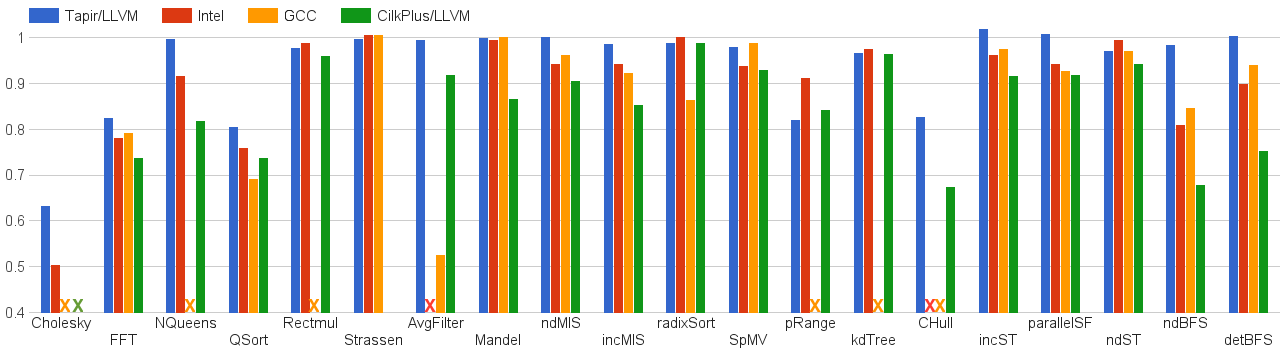
\includegraphics[width=\linewidth]{figures/chart.png}
% \begin{tab}{c}
% \bottomrule
% \end{tab}
% \caption{The work efficiency of mainstream compilers and \tapir/LLVM
%   on the Cilk Plus benchmarks described in \secref{eval}.  For each
%   compiler \tapir/LLVM, ICC 16.0.3, ICC 16.0.3, and GCC 5.3.0, the bar
%   for each benchmark shows the ratio $T_S/T_1$, where the serial
%   running time $T_s$ is running time of the benchmark when the Cilk
%   control constructs are replaced with their serial equivalents, and
%   the $1$-processor running time $T_1$ is the running time of the
%   parallel Cilk code on $1$ processor.  An X means that the compiler
%   failed to compile the code correctly, resulting in a runtime error.}
%   \label{fig:overhead}
% \end{figure*}

This thesis introduces \tapir, a compiler IR that represents logical
fork-join parallelism asymmetrically in the program's CFG\@.  The
asymmetry corresponds to the assumption of \defn{serial semantics}
\cite{FrigoLeRa98}, which means it is always semantically correct to
execute parallel tasks in the same order as an ordinary serial
execution.

\tapir adds three instructions --- \detach, \reattach, and \sync{} ---
to the IR of an ordinary serial compiler to express fork-join parallel
programs with serial semantics.  \subfigref{cfg}{d} illustrates the
\tapir CFG for the \code{fib} function.  As with the symmetric
parallel flow graph in \subfigref{cfg}{c}, \tapir places the logically
parallel recursive calls to \code{fib} in separate basic blocks.  But
these blocks do not join at a synchronization point symmetrically.
Instead, one block connects to the other, reflecting the serial
execution order of the program.

The \tapir approach provides five advantages:
\begin{closeenum}

\item Introducing fork-join parallelism into the compiler is
  relatively easy.

\item The IR is expressive and can represent fork-join control
  constructs from different parallel-language extensions.

\item \tapir parallel constructs harmonize with the invariants
  associated with existing representations of serial code.

\item Standard serial optimizations work on parallel code with few
  modifications.

\item The optimizations enabled by \tapir's parallelism constructs are
  effective in practice.

\end{closeenum}
I discuss each of these advantages in turn.

\section{Ease of implementation}

\tapir's asymmetric representation of logically parallel tasks makes
it relatively simple to integrate \tapir into an existing compiler's
intermediate representation such as LLVM IR~\cite{LLVMLangManual15}.
\figref{loc_breakdown} documents the lines of code added, modified, or
deleted to implement a prototype of \tapir in LLVM\@.  As
\figref{loc_breakdown} shows, \tapir/LLVM was implemented with about
$\fillintheblank{6000}$ lines, compared to LLVM's roughly
$\fillintheblank{4}$-million-line codebase.  Moreover, fewer than
$2000$ lines of code were needed to adapt LLVM's existing compiler
analyses and transformations to accommodate \tapir.

\begin{figure}[h!]
  %\setlength{\tabcolsep}{1pt}
  \small
  \sisetup{group-minimum-digits=4}
  \begin{tab}{lS[table-format=7.0]S[table-format=4.0]@{\hskip -2mm}l}
    \toprule
    \textit{Compiler Component} &
    \textit{LLVM 4.0svn} &
    \multicolumn{2}{l}{\textit{Tapir/LLVM}}
    \\
    \midrule
    Instructions            &  105 995 & 943 &
    \rdelim\}{3}{20pt}[$\num{1 768}$]  \\
    Memory Behavior         &  21 788  & 445 & \hspace{10mm}  \\
    Optimizations           &  152 229 & 380 &   \\
    Parallelism Lowering    &        0 & 3 782 & \\
    % Parallelism Lowering    &        0 & 1 774 & \\
    % New Parallel Optimizations   &        0  & 2 008   \\
    Other                   & 3 803 831  &  460     & \\
    \midrule
    Total                   & 4 083 843  &  6 010 &\\
    \bottomrule
  \end{tab}
  \caption[Code changes required to implement the \tapir/LLVM prototype.]{Breakdown of the lines of code added, modified, or deleted
    in LLVM to implement the \tapir/LLVM prototype.}
  \label{fig:loc_breakdown}
\vspace{-.4cm}
\end{figure}

The breakdown of lines is as follows.  The lines for ``Instructions''
add \tapir's instructions to LLVM IR and adapt LLVM's routines for
reading and writing LLVM IR and bitcode files.  Conceptually, these
changes allow LLVM to correctly compile a \tapir program to a serial
executable with no optimizations.  The lines for ``Memory Behavior''
control how \tapir instructions may interact with memory operations,
preventing the compiler from creating any races.  The lines for
``Optimizations'' perform any adjustments required for LLVM analyses
and transformations to compile a \tapir program at optimization
level~\code{-O3}.  Most of these modifications are not necessary for
creating a correct executable but are added to allow the compiler to
perform additional optimizations, such as parallel tail-recursion
elimination (described in \chapref{opt}).  The lines for ``Parallelism
Lowering'' translate \tapir instructions into Cilk Plus runtime calls
and allow the code to be race-detected with a provably good race
detector~\cite{FengLe99}.  The lines for ``Other'' address a bug in
LLVM's implementation of \code{setjmp} and implement useful features
for our development environment.

% \tbsnote{Technically, it's our own implementation
%   of SP-bags; it's not Cilkscreen:}the Cilk race detector
% Cilkscreen~\cite{Cilkscreen11}.

% Finally, the lines for ``New Parallel Optimizations'' implement new
% optimization passes specifically for parallel code.

\section{Expressiveness of \tapir}

\tapir can express logical fork-join parallelism in parallel programs
that have serial semantics.  For example, \figref{cfg} illustrates how
\tapir can express the parallelism encoded by the \CilkSpawn and
\CilkSync\ linguistics from Cilk++\ \cite{Leiserson10} and Cilk Plus
\cite{IntelCilkPlus10}, as well as the parallelism encoded by OpenMP
\code{task} and \code{taskwait} clauses~\cite{AyguadeCoDu09}.
Similarly, \tapir can express the parallelism encoded by OpenMP
parallel sections~\cite{OpenMP13} and Habanero's \code{async} and
\code{finish} constructs~\cite{CaveZhSh11}.  \tapir can also express
parallel loops, including \CilkFor loops and OpenMP parallel loops
that have serial semantics (described in \chapref{newir}).  Other
parallel constructs, such as those proposed in the C++17 parallelism extensions,
can be represented as well. However, parallel
operations that cannot be expressed in terms of fork-join parallelism,
such as OpenMP's \code{ordered} clause, cannot be represented directly
using \tapir's \detach, \reattach, and \sync instructions.

\tapir makes minimal assumptions about the consistency \cite{Pugh99,
  BoehmAd08} of concurrent memory accesses.  \tapir assumes that
memory is shared among parallel tasks and that virtual-register state
is local to each task.  Parallel instructions in \tapir can exhibit a
\defn{determinacy race}\footnote{Determinacy races are also called
  general races \cite{NetzerMi92} and are distinct from data races,
  which involve nonatomic accesses to critical regions.}
\cite{FengLe99} if they access the same memory location concurrently
and at least one instruction writes to that location.  \tapir itself
does not fully define the possible outcomes of a determinacy race, and
instead defers to existing compiler mechanisms, such as LLVM's atomic
memory-ordering constraints \cite{LLVMLangManual15}, to define
whichever memory model they choose.  For any targeted runtime system,
\tapir relies on a correct implementation of lowering in order to
implement the necessary synchronization, but \tapir is oblivious to
how that runtime system implements the synchronization.

\section{Serial semantics}

By grounding its model of parallelism in serial semantics, \tapir
enables common compiler optimizations for serial code to work on
parallel code.  Intuitively, because \tapir always allows parallel
tasks to execute in their ordinary serial execution order, the
compiler can to optimize parallel code in any manner that preserves
the serial semantics of the program and does not introduce new
determinacy races.  These mild constraints support common
optimizations on parallel code, such as sequentialization, which can
be invalid under models of parallelism without serial
semantics~\cite{VafeiadisBaCh15}.

\section{Optimizations}

In practice, the \tapir team has found that \tapir enables a wide variety of
standard compiler optimizations to work with parallel code.  The
prototype implementation of \tapir/LLVM, for example, successfully
moves the call to \code{norm} in \figref{normalize} outside of the
loop, just as it would for a serial \code{for} loop.  As \chapref{opt}
discusses, \tapir enables other optimizations, including
common-subexpression elimination \cite[Sec.~12.2]{Muchnick97},
loop-invariant-code motion \cite[Sec.~13.2]{Muchnick97}, and
tail-recursion elimination \cite[Sec.~15.1]{Muchnick97}, to work on
parallel code.  \tapir also enables new optimizations on parallel
control flow.

\begin{figure*}[t]
\begin{tab}{c}

\toprule
\end{tab}
  \begin{flushleft}
      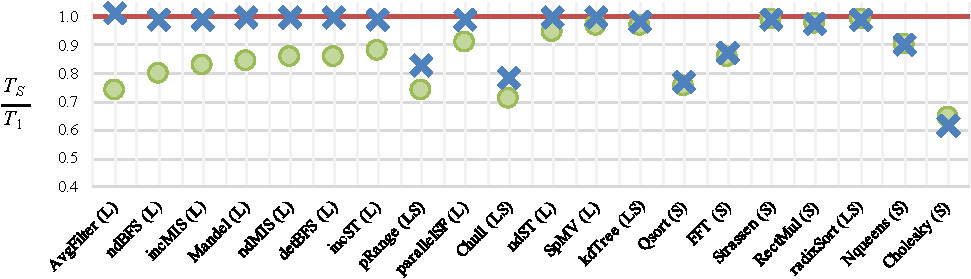
\includegraphics[width=\linewidth]{figures/workeff_scatter.pdf}
  \end{flushleft}
  \vspace*{-5mm}
  \begin{tab}{c}
  \bottomrule
 \end{tab}
 \caption[Graph of work efficiency comparison between Reference and Tapir/LLVM.]{Comparison of the work efficiency of
   \protect\fillintheblank{20} parallel application benchmarks
   compiled using \tapir/LLVM (X's) and the comparable Reference
   compiler (O's), described in \chapref{eval}, which lowers
   parallelism in the compiler front end.  Each point plots the work
   efficiency $T_S/T_1$ of a compiled benchmark, where $T_1$ is the
   work of the benchmark and $T_s$ is the running time of the serial
   elision of the benchmark.  Higher values indicate better work
   efficiency.  The horizontal line at $1.0$ plots the theoretically
   maximum work efficiency $T_S/T_1 = 1$.  Benchmarks are sorted by
   decreasing difference in work efficiency between \tapir/LLVM- and
   Reference-compiled executables.  Benchmarks marked with an ``L''
   use parallel loops, and benchmarks marked with an ``S'' use
   \CilkSpawn.}
  \label{fig:work_efficiency}
\end{figure*}

\section{Evaluation of \tapirllvm}

The compiler optimizations that \tapir enables are effective in
practice.  We evaluated the \tapir approach by measuring the
performance of \fillintheblank{20} Cilk application benchmarks
compiled using \tapirllvm.  We compared the performance of these
executables to those produced by a comparable reference compiler,
called Reference.  Conceptually, Reference lowers parallel linguistic
constructs directly into runtime calls, as mainstream compilers do
today, but otherwise performs the same set of optimization passes as
\tapirllvm.  \chapref{eval} describes our experimental setup in detail,
including the design of Reference.

\figref{work_efficiency} presents the results of comparing \tapirllvm
and Reference in terms of the ``work efficiency'' of the compiled
benchmarks.  To perform this comparison, We compiled each benchmark
using each compiler and then ran the executable on a single processing
core of a multicore machine to measure its \defn{work}, the $1$-core
running time, denoted~$T_1$.  We also used each compiler to compile,
run, and measure the $1$-core running time of the \defn{serial
  elision} \cite{FrigoLeRa98} of each benchmark, denoted $T_S$, in
which the benchmark is converted into a corresponding serial program
by replacing all parallel linguistic constructs with their serial
equivalents.  We then computed the \defn{work efficiency} of each
compiled benchmark, which is the ratio $T_S/T_1$ of the running time
$T_S$ of the benchmark's serial elision divided by the work $T_!$ of
the benchmark.  In theory, the maximum possible work efficiency is
$T_S/T_1 = 1$, but in practice, quirky behaviors of the compiler and
multicore architecture can occasionally produce work efficiencies
greater than~$1$.  As \figref{work_efficiency} shows, for most
benchmarks, the executables compiled using \tapir/LLVM achieve equal
or higher work efficiency than those compiled using Reference.
Moreover, for many benchmarks, and particularly those implemented
using parallel loops, \tapir/LLVM produces executables that achieve
nearly optimal work efficiency.  \chapref{eval} elaborates on these
experiments.

% \tbsnote{I feel the following assessment undersells our results a bit.
%   We should have some more space to expand the discussion of
%   results.}As \figref{work_efficiency} shows, across nearly all of the
% benchmark programs, \tapirllvm produces executables with equal or
% higher work efficiency than the Reference pipeline, validating the
% \tapir approach.

\section{Contributions} 

This thesis makes the following research contributions:
\begin{closeitemize}

\item The design of a compiler IR that represents fork-join
  parallelism asymmetrically, which enables existing serial
  optimizations to operate on parallel code and which also enables
  parallel optimizations.

\item The implementation of \tapir/LLVM in the LLVM compiler by
  modifying about $\fillintheblank{6000}$ source lines of code
  ($\fillintheblank{0.15\%}$ of the $4$-million-line LLVM codebase).

\item The implementation of parallel optimizations such as unnecessary
  synchronization elimination and parallel-loop scheduling.

\item Experiments that demonstrate the advantage of embedding
  fork-join parallelism into a compiler's IR, as opposed to dealing
  with parallelism only in the compiler's front end.

\end{closeitemize}


\section{Outline}

The remainder of this thesis is organized as follows.  \chapref{newir}
describes \tapir's representation and properties.  \chapref{analyses}
discusses how analysis passes can be adapted to operate on \tapir
programs.  \chapref{opt} describes various optimizations on parallel
control flow that \tapir enables.  \chapref{aux} describes auxiliary
software we developed to exercise and test \tapir/LLVM\@.
\chapref{eval} discusses our evaluation of the effectiveness of \tapir.
\chapref{related} discusses related work.  \chapref{concl} provides some
concluding remarks.  An appendix describes how to set up \tapir/LLVM
and how to download and run our suite of application benchmarks.
